\documentclass{article} \usepackage{amsmath} \usepackage{amssymb} \usepackage{amsthm} \usepackage[margin=0.2in]{geometry} \usepackage{hyperref} \usepackage{physics} \usepackage{tikz} \usepackage{mathtools} \mathtoolsset{showonlyrefs} \theoremstyle{definition} \newtheorem{theorem}{Theorem}[section] \newtheorem{corollary}{Corollary}[theorem] \newtheorem{lemma}[theorem]{Lemma} \newtheorem{definition}{Definition}[section] \author{Connor Duncan} \date{\today}
\title{Physics-105-Lecture-Notes-04-02-2019}
\begin{document}
\maketitle\tableofcontents
\noindent\abstract{A single PDF with all lectures in a single document can be downloaded at \url{https://www.dropbox.com/sh/8sqzvxghvbjifco/AAC9LoSRnsRQDp7pYedgWpQMa?dl=0}. The password is 'analytic.mech.dsp'.
 This file was automatically generated using a script, so there might be some errors. If there are, you can contact me at \url{mailto:ctdunc@berkeley.edu}.}
\subsection{Euler Angles, Body/Space Frames} The beginning of lecture was some complicated example using the euler angles to transform into body coordinates. Here's another version of this problem. \subsubsection{Symmetric Top} We have $I_1=I_2=I$. It can be a cube, or really something arbitrary. $I_3$ might be different. KE can be written $T=\frac{1}{2}\vec{\omega}(I\cdot\vec{\omega})=\frac{1}{2}(I(\omega_1^2+\omega_2^2)+I_3\omega_3^2)$. Using this, and the formulation of the euler angles, we can write down htat \begin{align} \omega_1^2=\dot\theta^2\cos^2\chi+\dot\varphi^2\sin^2\chi\sin^2\theta+2\dot\theta\dot\varphi\cos\chi\sin\chi\sin\theta \end{align} with omega 2 defined in a similar manner, which gives \begin{align} \omega_1^2+\omega_2^2=\dot\theta^2+\dot\varphi^2\sin^2\theta\\ \omega_3^2=(\dot\chi+\dot\varphi\cos\theta)^2 \end{align} In gravity, there's also potential $V=mgl\cos\theta$, so we can write down the lagrangian \begin{equation} \mathcal L=\frac{I}{2}(\dot\theta^2+\dot\varphi^2\sin^2\theta)+\frac{I_3}{2}(\dot\chi+\dot\varphi\cos\theta)^2-mgl\cos\theta \end{equation} From our work on canonical variables, we can note that \begin{align} p_\varphi=\text{constant} \\ p_\chi=\text{constant} \end{align} we can calculate these then, as \begin{align} p_\chi=\pdv{\mathcal L}{\dot\chi}=I_3(\dot\chi+\dot\varphi\cos\theta)=I_3\omega_3 \end{align} Which is angular momentum around $x_3$. Also, define $a=\frac{I_3\omega_3}{I}\equiv$const. Now, we can calculate \begin{equation} p_\varphi=\pdv{\mathcal L}{\dot\varphi}=I\dot\varphi\sin^2\theta+I_3(\dot\chi+\dot\varphi\cos\theta)\cos\theta\equiv\text{constant} \end{equation} Define $b=\frac{p_\varphi}{I}$. We can calculate the total energy then as \begin{align} E=T+U=\frac{I_2}{2}(\dot\theta^2+\dot\varphi^2\sin^2\theta)+\frac{I_3}{2}\omega_3^2+Mgl\cos\theta \end{align} This whole equation simplifies down to a nice form, which is $b=\dot\varphi\sin^2\theta+a\cos\theta$. If we wirte $E'=E-\frac{I_3\omega_3^2}{2}$, then we can have a one-dimensoinal equation \begin{equation} E'=\frac{I}{2}\dot\theta^2+\frac{I}{2}\frac{(b-a\cos\theta)^2}{\sin^2\theta}+mgl\cos\theta \end{equation} We can look at this like an energy equation \begin{center} 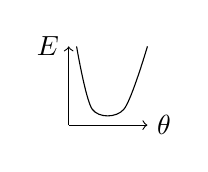
\begin{tikzpicture} \draw[->] (0,0)--(1,0) node[anchor=west]{$\theta$}; \draw[->] (0,0)--(0,1) node[anchor=east]{$E$}; \draw plot [smooth] coordinates {(0.1,1)(0.3,0.2)(0.7,0.2)(1,1)}; \end{tikzpicture} \end{center} If we define $\dot\theta^2(1-u^2)=\dot u^2$, we can do some fancy substitution. As $u\rightarrow\infty$, everythign goes as $u^3$. Likewise for $-\infty$. If we now consider $\dot\varphi=\frac{b-a\cos\theta}{\sin^2\theta}$, we can see that it will not have zero average. In fact, it will look like some curly path between these two lines on a sphere. \begin{center} 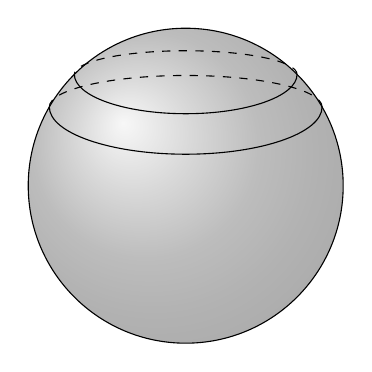
\begin{tikzpicture} \shade[ball color=gray, opacity =0.4] (0,0) circle (2cm); \draw (0,0) circle (2cm); \draw ({2cm*cos(45)},{2cm*sin(45)})arc(360:180:{2*cos(45)} and 0.5); \draw[dashed] ({2cm*cos(45)},{2cm*sin(45)})arc(0:180:{2*cos(45)} and 0.3); \draw ({2cm*cos(30)},{2cm*sin(30)})arc(360:180:{2*cos(30)} and 0.6); \draw[dashed] ({2cm*cos(30)},{2cm*sin(30)})arc(0:180:{2*cos(30)} and 0.4); \end{tikzpicture} \end{center}
\end{document}
